\section{QFT, XY routing}
11076 hops; seeds 60, 61; every run completed every hop and passed the physical audit (Checks sheet of the workbook).
\subsection{Headline: 8 memories per core, 6 for pre-generation}
ODG, CGP, ACGP and Dynamic~(8) use 8 memories per core, of which 6 may hold pre-generated pairs; Dynamic~($\infty$) uses 64, which no core ever fills.
\begin{table}[H]\centering\small
\begin{tabular}{lrrrrrrr}\toprule
Configuration & Latency (ms) & p95 (ms) & Fidelity & Hop cov. (\%) & Chain full (\%) & Wastage (\%) & Utilisation (\%)\\\midrule
ODG & 1.782 & 4.60 & 0.9498 & 0.0 & 0.0 & -- & --\\
CGP & 0.970 & 3.25 & 0.9424 & 77.9 & 60.1 & 4.24 & 95.8\\
ACGP & 0.976 & 3.30 & 0.9421 & 77.6 & 60.0 & 4.39 & 95.6\\
Dynamic (8) & 0.747 & 2.25 & 0.9439 & 76.8 & 64.5 & 1.23 & 98.8\\
Dynamic ($\infty$) & 0.616 & 1.65 & 0.9442 & 84.0 & 71.9 & 1.18 & 98.8\\
\bottomrule\end{tabular}
\caption{QFT, XY routing, 8 memories per core, 6 for pre-generation: mean of the seeds.}\end{table}
\begin{figure}[H]\centering
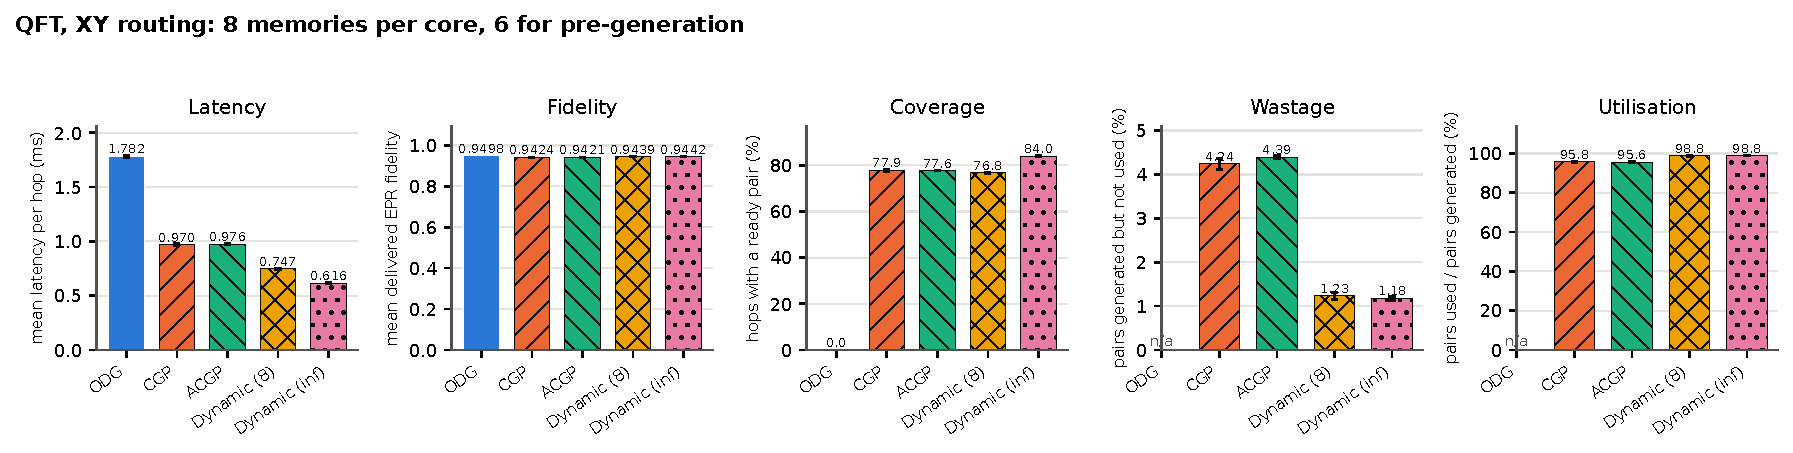
\includegraphics[width=\linewidth]{qft_xy_headline_8.pdf}
\caption{QFT, XY routing, 8 memories per core, 6 for pre-generation. Bars are the mean of the seeds, whiskers the seed range; fidelity bars start at zero, so read the labels.}\end{figure}
\subsection{Headline: 4 memories per core, all 4 for pre-generation}
ODG, CGP, ACGP and Dynamic~(4) use 4 memories per core and ODG and Dynamic may use all 4 for pre-generation; CGP and ACGP cache at most 3 (all 4 starves them), the same as in the $K$ sweep; Dynamic~($\infty$) as above.
\begin{table}[H]\centering\small
\begin{tabular}{lrrrrrrr}\toprule
Configuration & Latency (ms) & p95 (ms) & Fidelity & Hop cov. (\%) & Chain full (\%) & Wastage (\%) & Utilisation (\%)\\\midrule
ODG & 1.887 & 4.80 & 0.9498 & 0.0 & 0.0 & -- & --\\
CGP & 2.331 & 8.95 & 0.9401 & 63.0 & 41.7 & 5.87 & 94.1\\
ACGP & 2.325 & 8.95 & 0.9402 & 63.4 & 43.9 & 5.76 & 94.2\\
Dynamic (4) & 1.295 & 4.70 & 0.9425 & 63.7 & 54.1 & 3.89 & 96.1\\
Dynamic ($\infty$) & 0.616 & 1.65 & 0.9442 & 84.0 & 71.9 & 1.18 & 98.8\\
\bottomrule\end{tabular}
\caption{QFT, XY routing, 4 memories per core, all 4 for pre-generation: mean of the seeds.}\end{table}
\begin{figure}[H]\centering
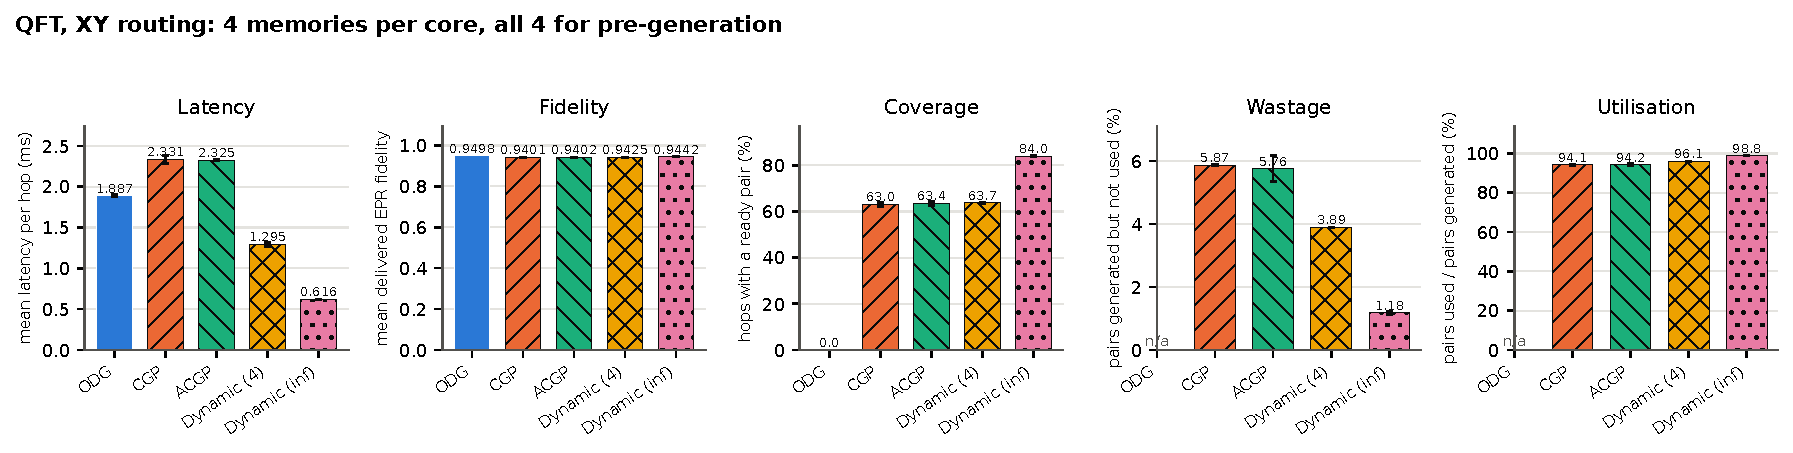
\includegraphics[width=\linewidth]{qft_xy_headline_4all.pdf}
\caption{QFT, XY routing, 4 memories per core, all 4 for pre-generation. Bars are the mean of the seeds, whiskers the seed range; fidelity bars start at zero, so read the labels.}\end{figure}
\subsection{Memories per core K}
Dynamic may use all K memories, except 6 of 8 at $K=8$; CGP and ACGP cache $\lfloor 0.75K\rfloor$ pairs (so at $K=1$ they are ODG). $K=\infty$ is 64 memories.
\begin{table}[H]\centering\small
\begin{tabular}{lrrrrrrr}\toprule
Latency & $K=1$ & $K=2$ & $K=3$ & $K=4$ & $K=6$ & $K=8$ & $K=\infty$\\\midrule
ODG & 6.275 & 2.816 & 2.109 & 1.887 & 1.788 & 1.782 & 1.782\\
CGP & 6.275 & 4.177 & 2.885 & 2.331 & 1.237 & 0.970 & 0.457\\
ACGP & 6.275 & 4.118 & 2.974 & 2.325 & 1.247 & 0.976 & 0.458\\
Dynamic & 9.041 & 3.528 & 1.877 & 1.295 & 0.866 & 0.747 & 0.616\\
\bottomrule\end{tabular}
\caption{QFT, XY routing: latency (mean latency per hop (ms)) for every K.}\end{table}
\begin{figure}[H]\centering
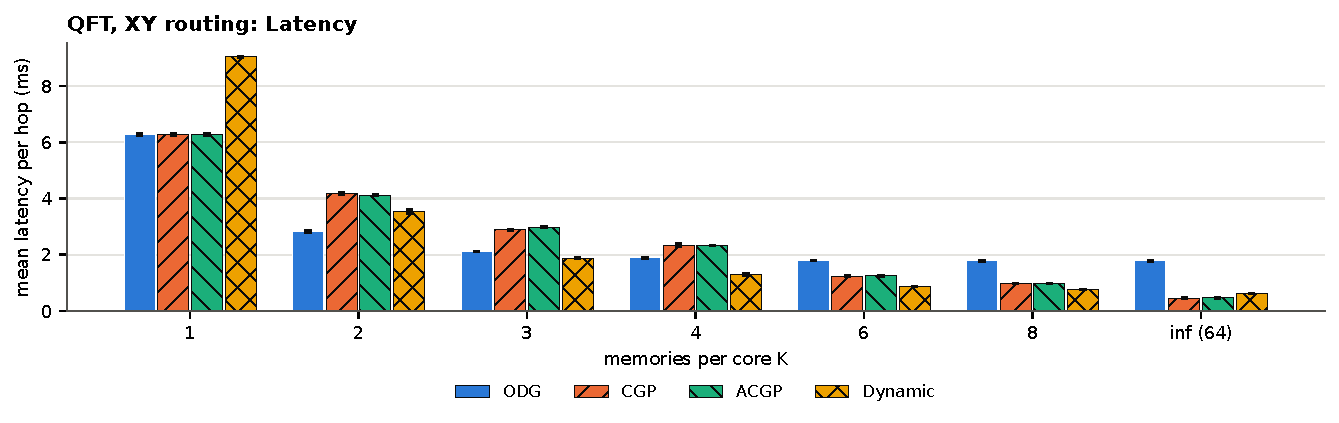
\includegraphics[width=\linewidth]{qft_xy_k_latency_ms.pdf}
\caption{QFT, XY routing: latency for every K.}\end{figure}
\begin{table}[H]\centering\small
\begin{tabular}{lrrrrrrr}\toprule
Fidelity & $K=1$ & $K=2$ & $K=3$ & $K=4$ & $K=6$ & $K=8$ & $K=\infty$\\\midrule
ODG & 0.9498 & 0.9498 & 0.9498 & 0.9498 & 0.9498 & 0.9498 & 0.9498\\
CGP & 0.9498 & 0.9441 & 0.9415 & 0.9401 & 0.9427 & 0.9424 & 0.9422\\
ACGP & 0.9498 & 0.9441 & 0.9414 & 0.9402 & 0.9425 & 0.9421 & 0.9422\\
Dynamic & 0.9486 & 0.9440 & 0.9429 & 0.9425 & 0.9432 & 0.9439 & 0.9442\\
\bottomrule\end{tabular}
\caption{QFT, XY routing: fidelity (mean delivered EPR fidelity) for every K.}\end{table}
\begin{figure}[H]\centering
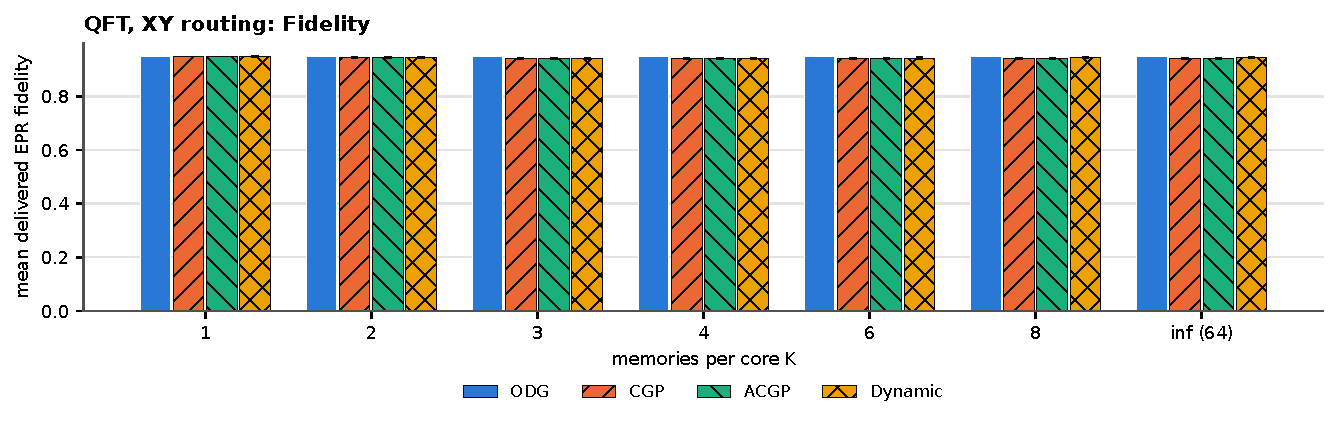
\includegraphics[width=\linewidth]{qft_xy_k_fidelity.pdf}
\caption{QFT, XY routing: fidelity for every K.}\end{figure}
\begin{table}[H]\centering\small
\begin{tabular}{lrrrrrrr}\toprule
Coverage & $K=1$ & $K=2$ & $K=3$ & $K=4$ & $K=6$ & $K=8$ & $K=\infty$\\\midrule
ODG & 0.0 & 0.0 & 0.0 & 0.0 & 0.0 & 0.0 & 0.0\\
CGP & 0.0 & 26.8 & 50.5 & 63.0 & 64.2 & 77.9 & 99.3\\
ACGP & 0.0 & 27.0 & 49.0 & 63.4 & 63.9 & 77.6 & 99.1\\
Dynamic & 8.9 & 36.3 & 52.4 & 63.7 & 76.8 & 76.8 & 84.0\\
\bottomrule\end{tabular}
\caption{QFT, XY routing: coverage (hops with a ready pair (\%)) for every K.}\end{table}
\begin{figure}[H]\centering
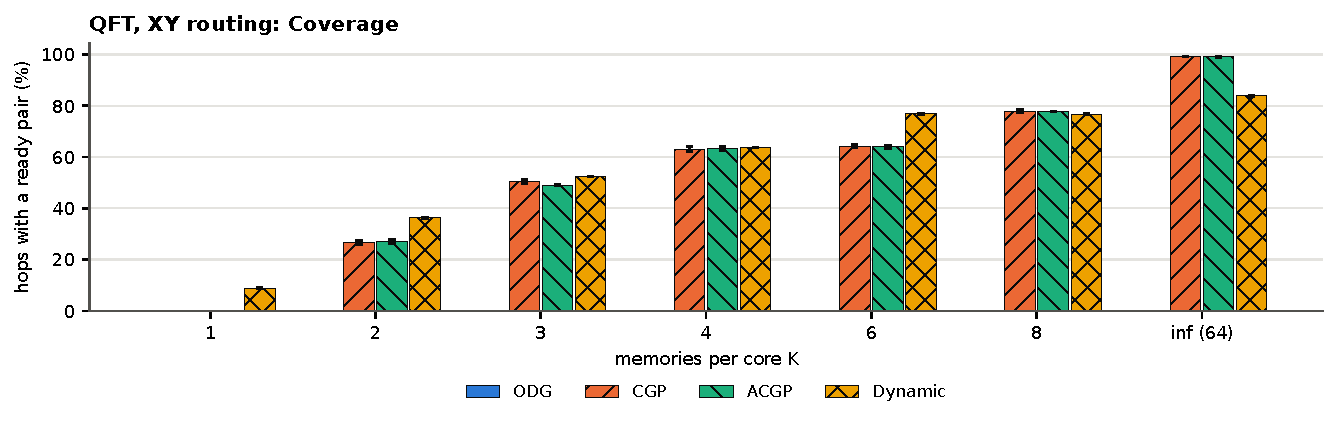
\includegraphics[width=\linewidth]{qft_xy_k_hop_coverage_pct.pdf}
\caption{QFT, XY routing: coverage for every K.}\end{figure}
\begin{table}[H]\centering\small
\begin{tabular}{lrrrrrrr}\toprule
Wastage & $K=1$ & $K=2$ & $K=3$ & $K=4$ & $K=6$ & $K=8$ & $K=\infty$\\\midrule
ODG & -- & -- & -- & -- & -- & -- & --\\
CGP & -- & 7.08 & 5.66 & 5.87 & 4.34 & 4.24 & 13.73\\
ACGP & -- & 7.04 & 6.13 & 5.76 & 4.49 & 4.39 & 13.73\\
Dynamic & 60.80 & 14.59 & 6.08 & 3.89 & 2.05 & 1.23 & 1.18\\
\bottomrule\end{tabular}
\caption{QFT, XY routing: wastage (pairs generated but not used (\%)) for every K.}\end{table}
\begin{figure}[H]\centering
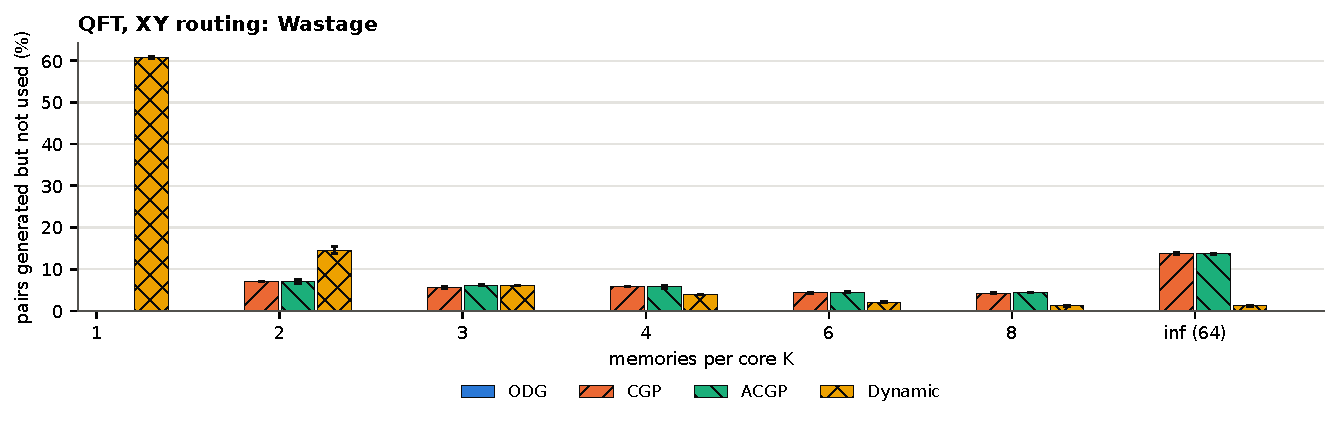
\includegraphics[width=\linewidth]{qft_xy_k_wastage_pct.pdf}
\caption{QFT, XY routing: wastage for every K.}\end{figure}
\begin{table}[H]\centering\small
\begin{tabular}{lrrrrrrr}\toprule
Utilisation & $K=1$ & $K=2$ & $K=3$ & $K=4$ & $K=6$ & $K=8$ & $K=\infty$\\\midrule
ODG & -- & -- & -- & -- & -- & -- & --\\
CGP & -- & 92.9 & 94.3 & 94.1 & 95.7 & 95.8 & 86.3\\
ACGP & -- & 93.0 & 93.9 & 94.2 & 95.5 & 95.6 & 86.3\\
Dynamic & 39.2 & 85.4 & 93.9 & 96.1 & 98.0 & 98.8 & 98.8\\
\bottomrule\end{tabular}
\caption{QFT, XY routing: utilisation (pairs used / pairs generated (\%)) for every K.}\end{table}
\begin{figure}[H]\centering
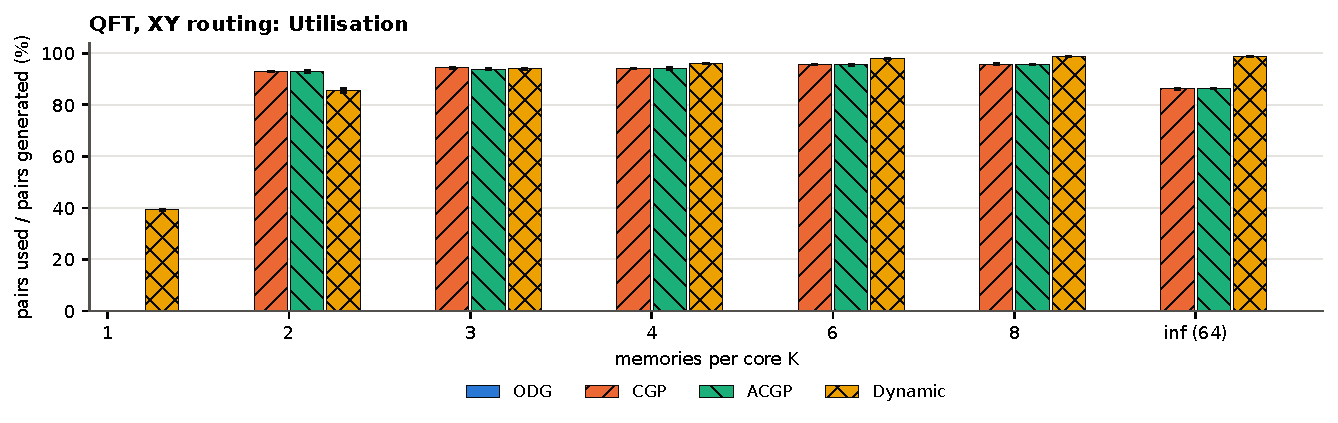
\includegraphics[width=\linewidth]{qft_xy_k_utilisation_pct.pdf}
\caption{QFT, XY routing: utilisation for every K.}\end{figure}
